\documentclass[landscape]{article}
\usepackage{ulem}
\usepackage[pdftex]{graphicx}
\pagestyle{empty}
\oddsidemargin  -0.5 in
\evensidemargin -0.5 in
\headheight     0 in
\topmargin      -1 in
\textheight     7.7 in
\textwidth      10 in
\begin{document}
\huge
\renewcommand{\labelitemi}{-}
\setlength{\parindent}{0 cm}

\begin{figure}[!ht]
  \begin{center}
    \begin{tabular}{p{0.49\linewidth} p{0.49\linewidth}}
      \begin{minipage}{\linewidth} \begin{center} Electrons left-polarized 95\% \end{center} \end{minipage} &
      \begin{minipage}{\linewidth} \begin{center} Electrons right-polarized 95\% \end{center} \end{minipage} \\
      \begin{minipage}{\linewidth} 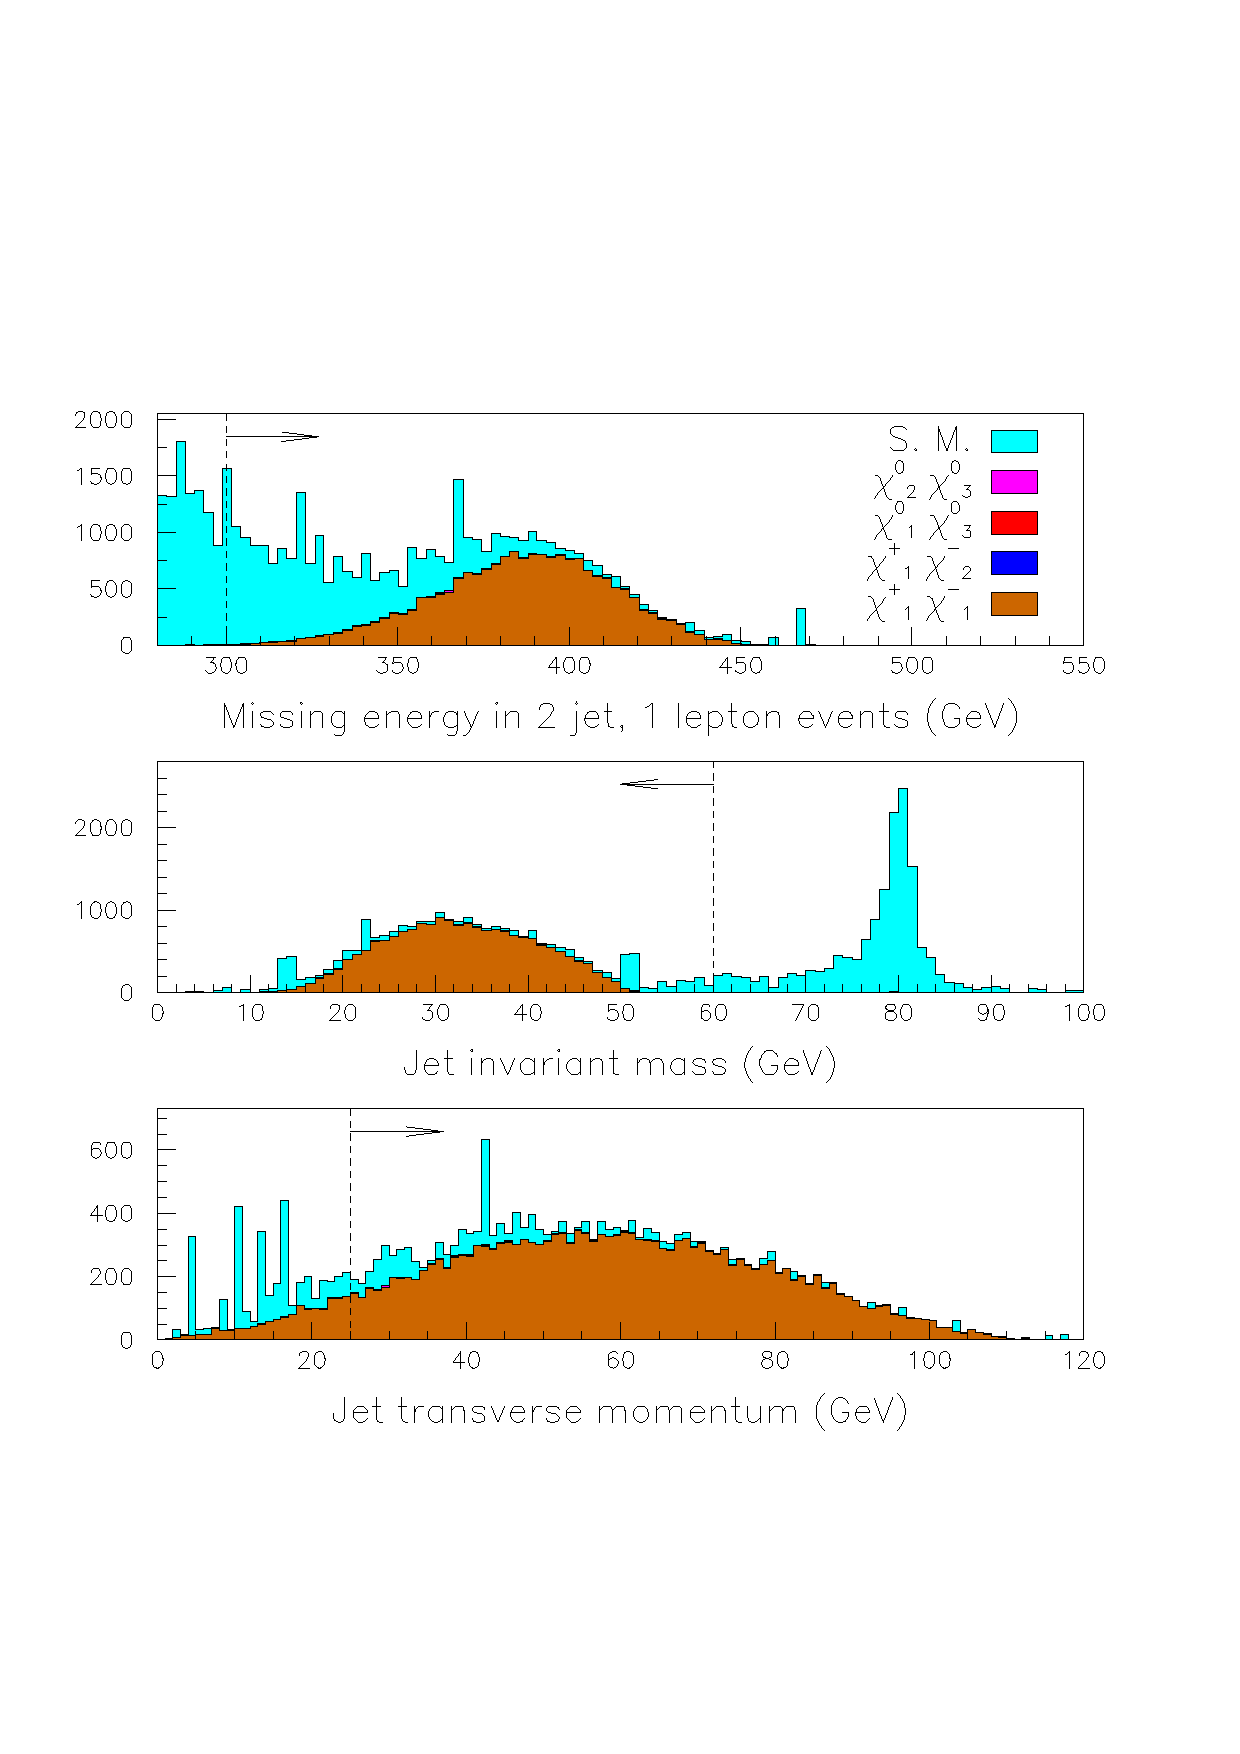
\includegraphics[width=\linewidth]{charginos_left.pdf} \end{minipage} &
      \begin{minipage}{\linewidth} \includegraphics[width=\linewidth]{charginos_right.pdf} \end{minipage}
    \end{tabular}

    \caption{\large Three cuts used to define $\chi_1^+\chi_1^-$ events, top
    to bottom: missing energy $>$ 300 GeV, di-jet invariant mass $<$
    60 GeV, and missing transverse jet momentum $>$ 25 GeV, applied
    cumulatively.  The plots on the left show 250 fb$^{-1}$ with
    electrons left-polarized, the ones on the right show 250 fb$^{-1}$
    with electrons right-polarized.  Brown is signal, light blue is
    all Standard Model background.  SUSY backgrounds are negligible
    for this mode.}

    \label{jimpcharginocuts}
  \end{center}
\end{figure}

Jets and leptons must be within $|\cos\theta| <$ 0.95.

My backgrounds are {\it not} two-photon; they are $e^+e^- \to
\ell^+\ell^- \nu \bar{\nu} Q \bar{Q}$ (\#44, \#48) and $\to q \bar{q}
b \bar{b} b \bar{b}$ (\#50) (where $q$ = $u$, $d$, $c$, $s$, and $Q$ =
$u$, $d$, $c$, $s$, $b$).

\pagebreak

What's in my simulation?

\begin{itemize}

\item Initial state radiation

\item All kinematics of decaying particles (including off-shell $W^\pm$ masses from Andreas's function)

\item Kinematic cuts that matter: $|\cos \theta| <$ 0.95 for jets and lepton, missing transverse jet momentum

\item \sout{Efficiency loss due to jet-confused lepton}

\item \sout{Jet invariant mass smearing (from $Z^0$ jet invariant mass distribution)}

\item Two-dimensional fit to jet-jet mass/total jet energy

\item Data has errors inflated by (completely unbiased) background subtraction

\end{itemize}

\vfill

Comparison is now made between generator-level quarks and my model,
{\it not} reconstructed jets and my model.

\vfill

\begin{center}
\begin{minipage}{0.5\linewidth}
\begin{itemize}\renewcommand{\labelitemi}{\mbox{ }}

  \item $\zeta$ = $\displaystyle \frac{|C_V|^2 - |C_A|^2}{|C_V|^2 + |C_A|^2}$ = 1 $\pm$ 0.0065

  \item $m_{\chi_1^\pm}$ = 159.4 $\pm$ 1.5 GeV (no bias!)

  \item $m_{\mbox{\large LSP}}$ = 107.7 $\pm$ 1.4 GeV (no bias!)

\end{itemize}
\end{minipage}
\end{center}

\pagebreak

What came out?  (These are projections of the 2-D distribution.)

\vfill

\begin{center} 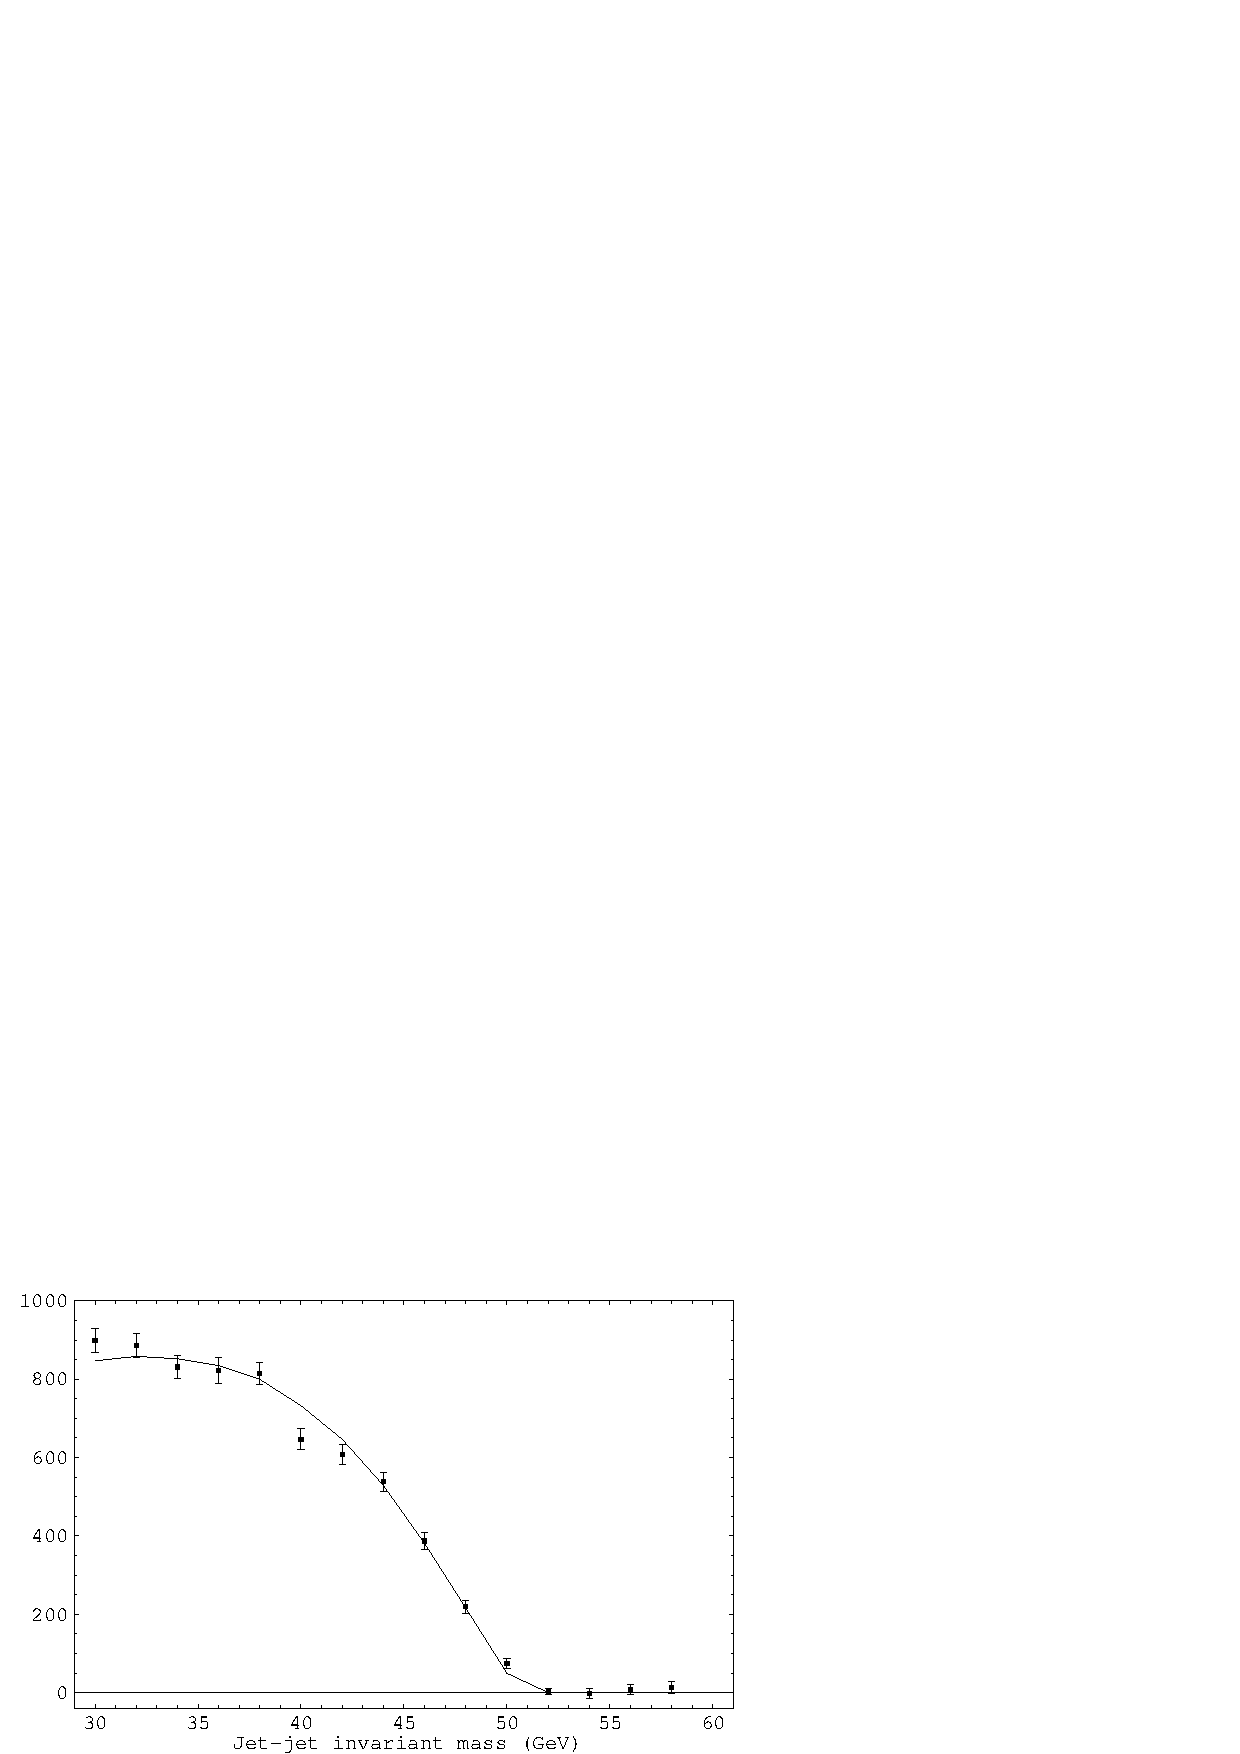
\includegraphics[width=0.5\linewidth]{fakeit2_mass.pdf} \end{center}

\vfill

\begin{center} 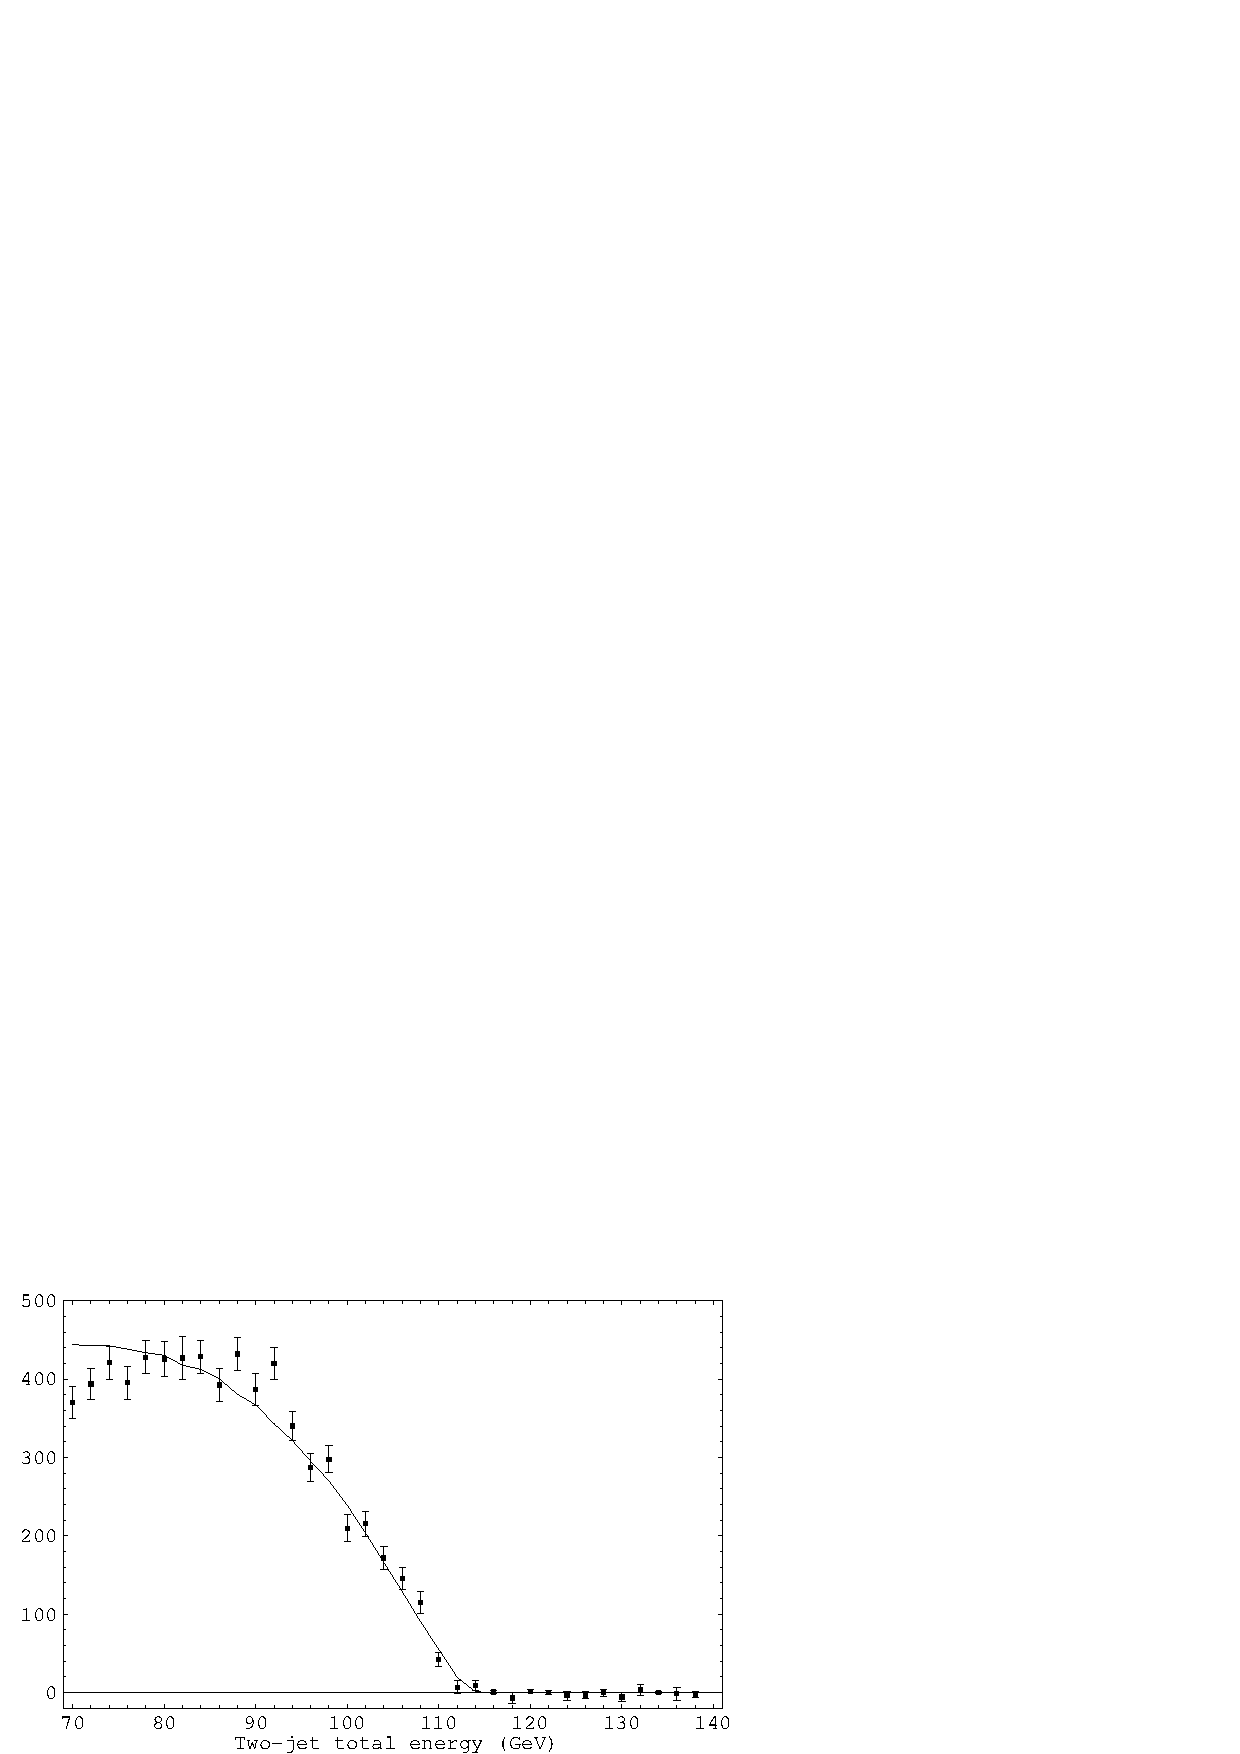
\includegraphics[width=0.5\linewidth]{fakeit2_energy.pdf} \end{center}

\pagebreak

What came out?  (Yellow was not calculated: I underestimated the time it would take to compute this.  One to three sigmas are shown with contours.)

\vfill

\begin{center}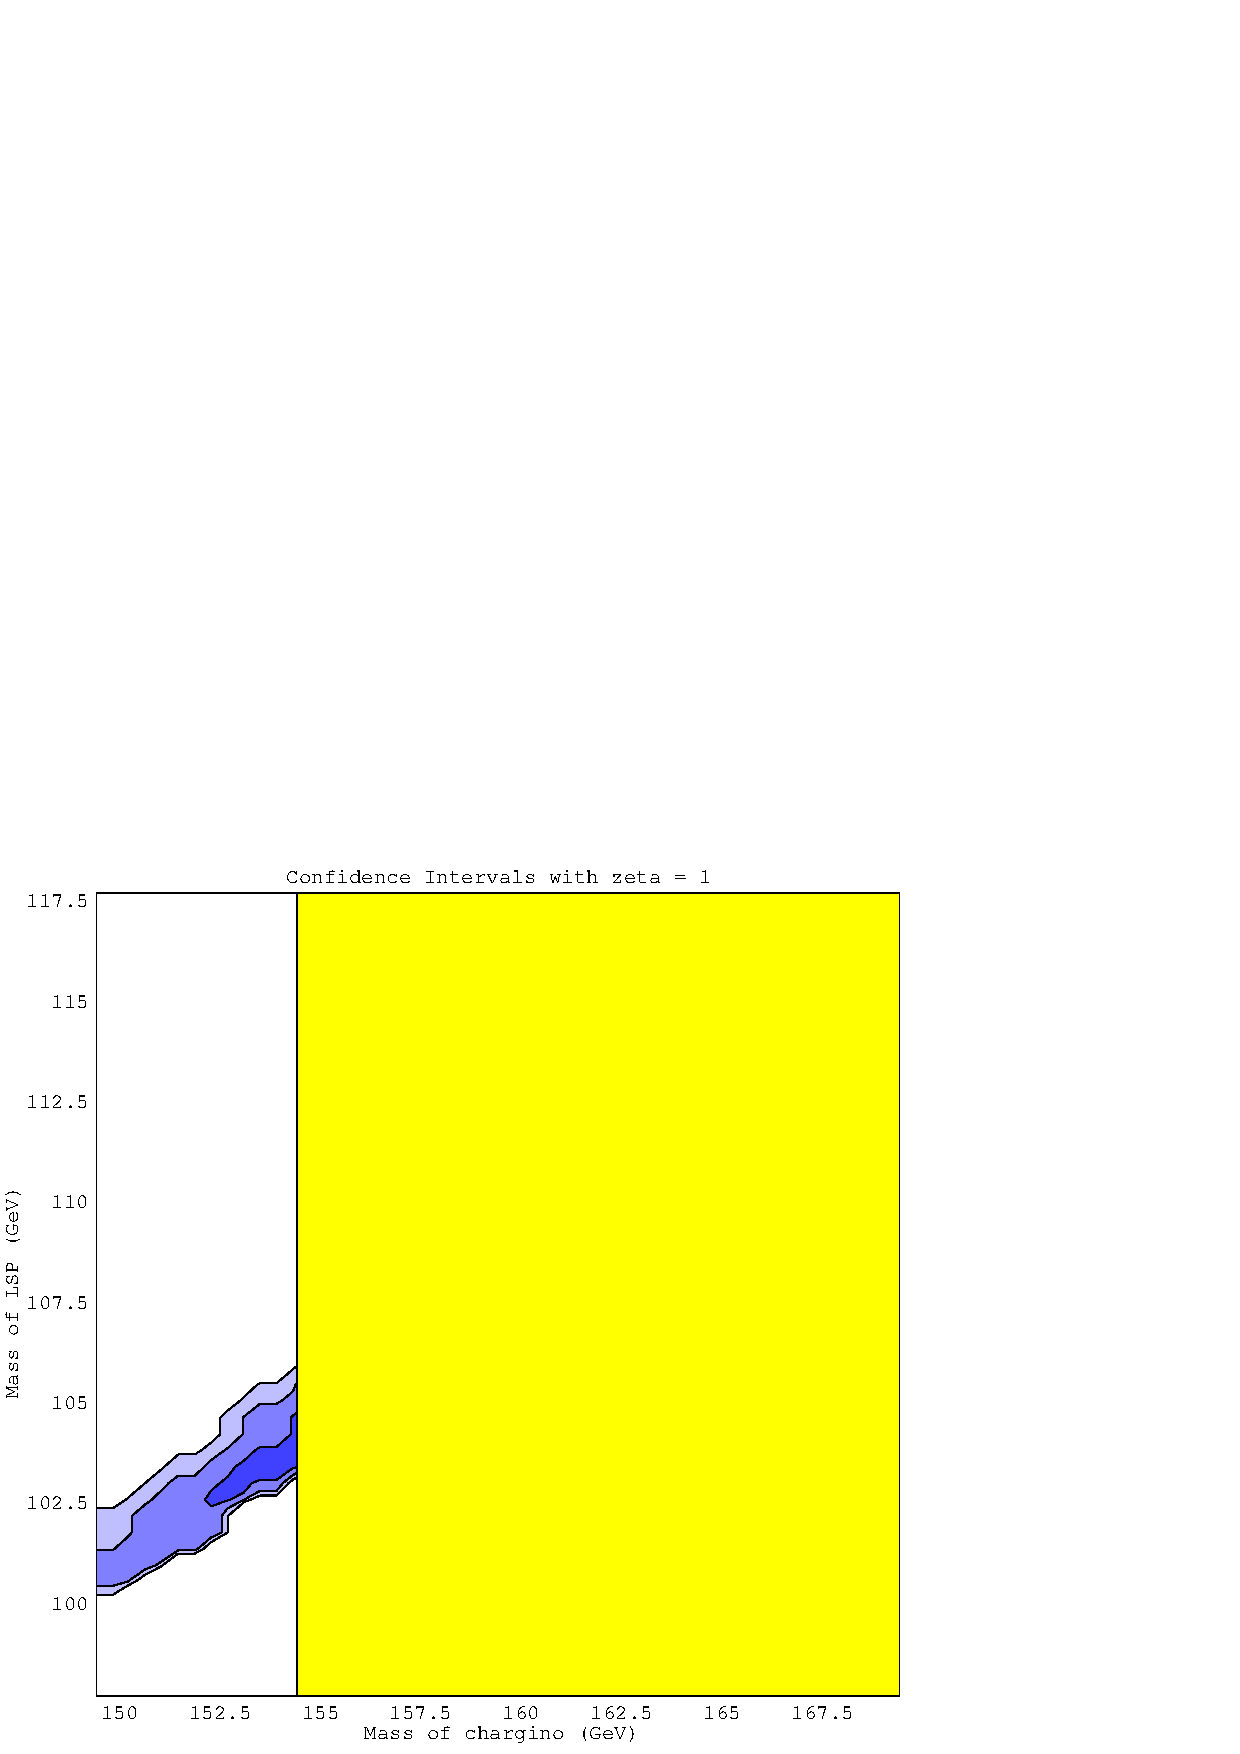
\includegraphics[width=0.7\linewidth]{fakeit2_chisquare_tmpbowl.pdf}\end{center}

\pagebreak

What came out?  (Yellow was not calculated: this is a 2-D projection of the initial quick scan from which I derived uncertainties.  One to three sigmas are shown with contours.)

\vfill

\begin{center}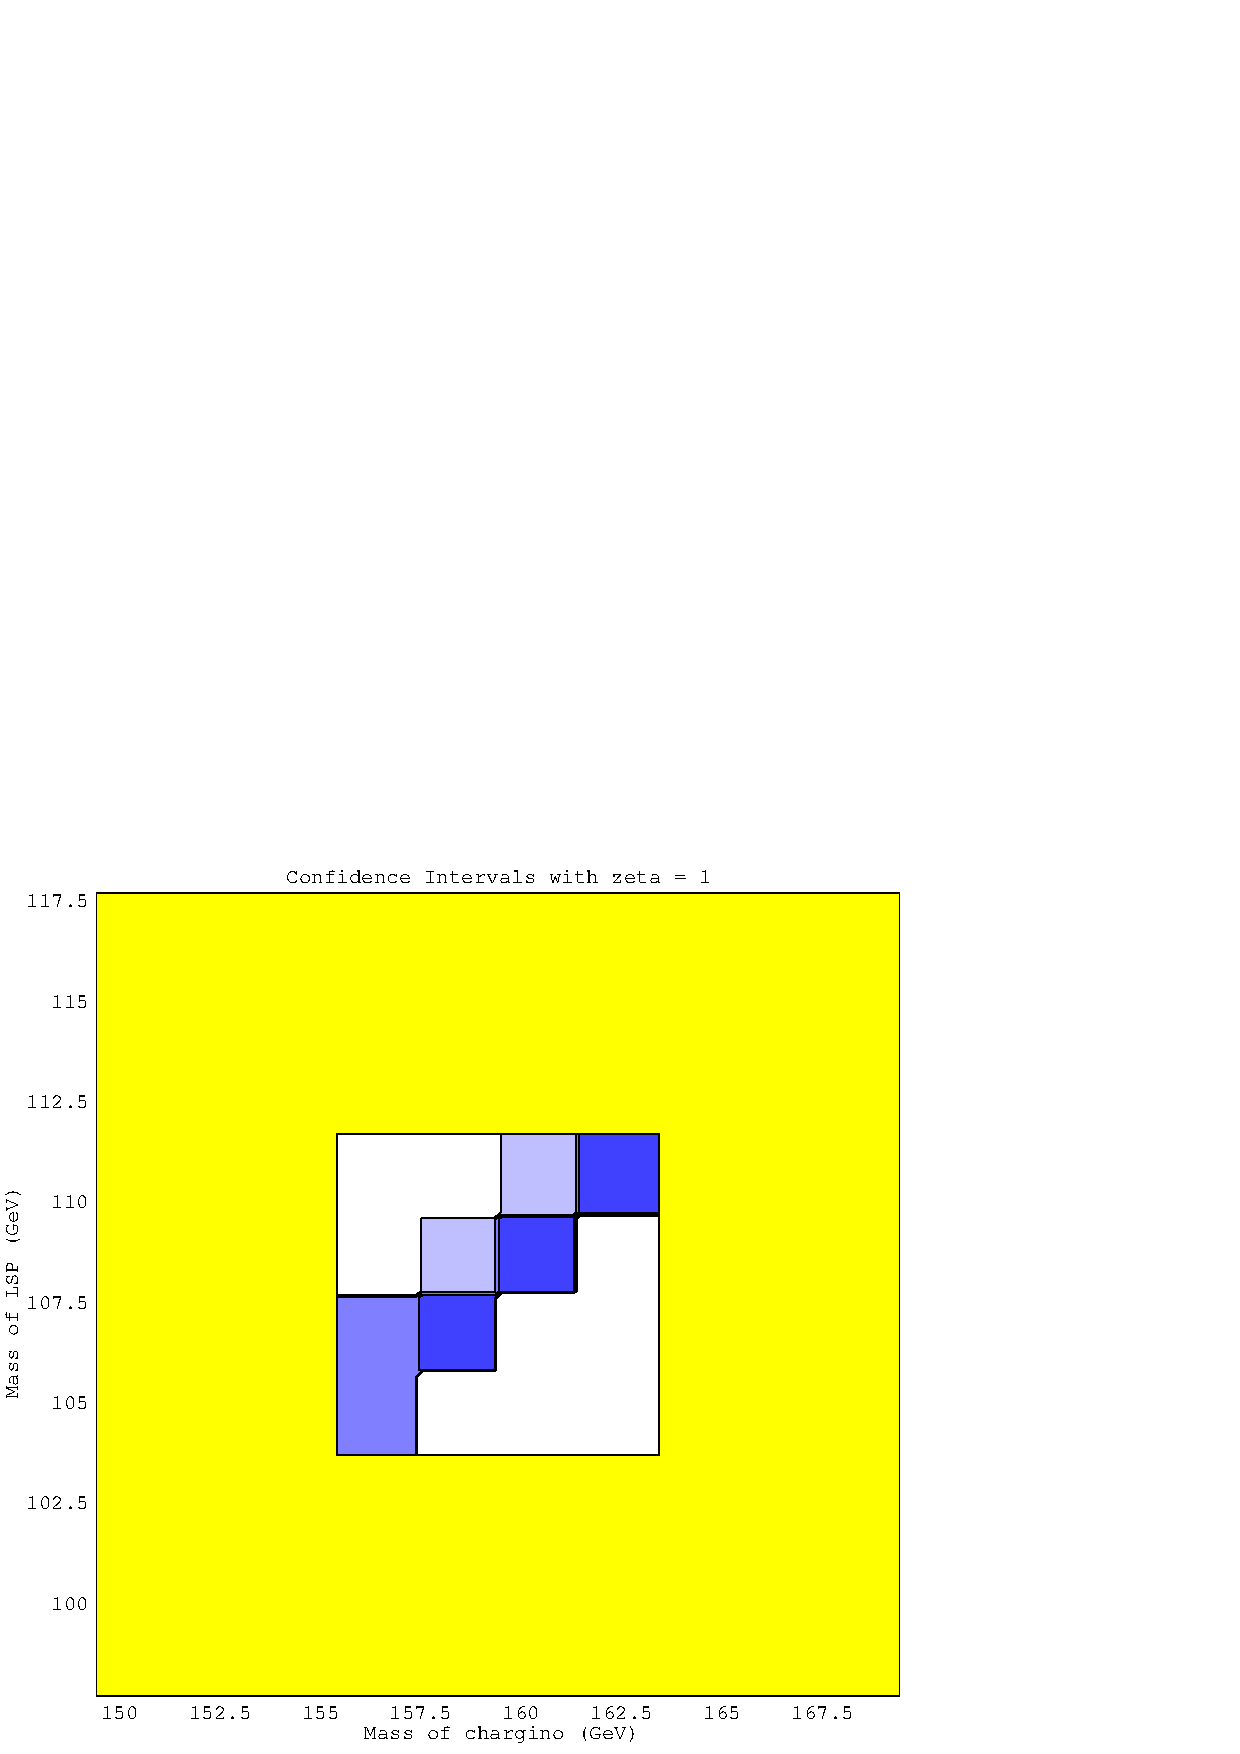
\includegraphics[width=0.7\linewidth]{fakeit2_chisquare_tmpbowl2.pdf}\end{center}

\end{document}
